\subsection{Filterkurve des Selektivfilters}
Die Ausgangsspannung $U_A$ wird in Abhängigkeit der Frequenz $f$ gemessen.
Die Messwerte sind in Tabelle \ref{tab:Q} zu finden.
Sie sind in Abbildung \ref{fig:Q} aufgetragen.
\begin{table}[h!]
  \centering
  \caption{Ausgangsspannung $U_A$ in Abhängigkeit von der Frequenz $f$}
  \label{tab:Q}
  \begin{tabular}{c c c c}
    \toprule
      $f$/kHz & $U_A$/V & $f$/kHz  & $U_A$/V  \\
    \midrule
    20    &   0,0432    &   34,5  &   0,5120 \\
    21    &   0,0480    &   34,6  &   0,5280  \\
    22    &   0,0528    &   34,8  &   0,5360  \\
    23    &   0,0584    &   35    &   0,5520  \\
    24    &   0,0648    &   35,1  &   0,5600  \\
    25    &   0,0728    &   35,2  &   0,5600  \\
    26    &   0,0816    &   35,3  &   0,5600  \\
    27    &   0,0928    &   35,4  &   0,5600  \\
    28    &   0,1040    &   35,5  &   0,5600  \\
    29    &   0,1240    &   35,6  &   0,5440  \\
    30    &   0,1480    &   35,7  &   0,5440  \\
    31    &   0,1820    &   35,8  &   0,5280  \\
    32    &   0,2320    &   36    &   0,5040  \\
    33    &   0,3120    &   37    &   0,3840  \\
    33,5  &   0,3640    &   38    &   0,3040  \\
    34    &   0,4480    &   39    &   0,2480  \\
    34,2  &   0,4640    &   40    &   0,1840  \\
    34,4  &   0,5040    &   -     &   -       \\

    \bottomrule
  \end{tabular}
\end{table}

\begin{figure}[h!]
  \centering
  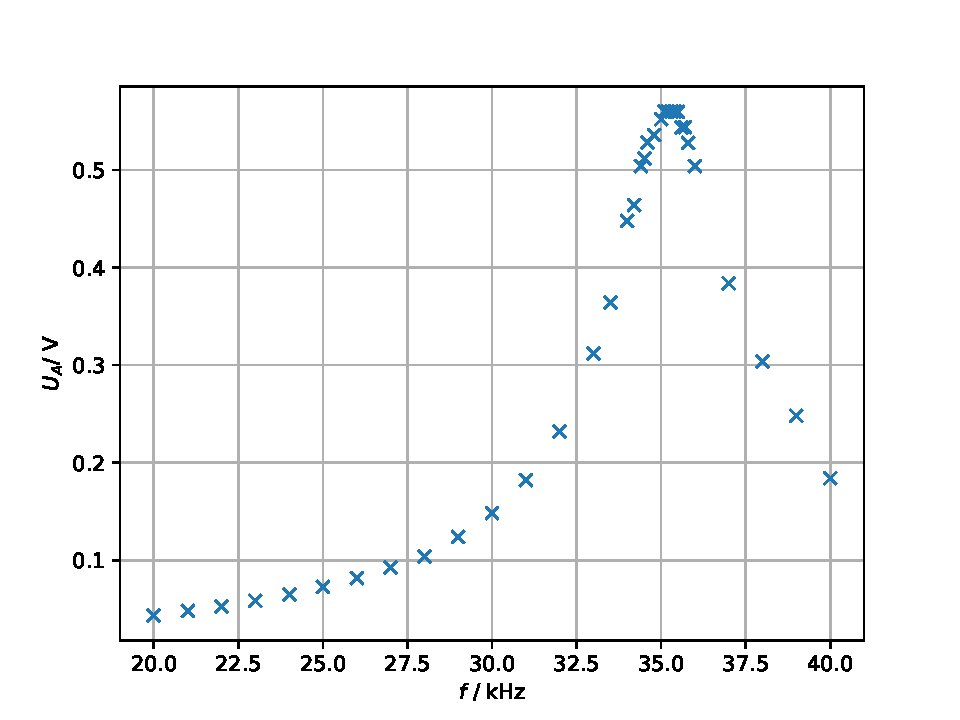
\includegraphics[width=\textwidth]{Q.pdf}
  \caption{Ausgangsspannung $U_A$ gegen Frequenz $f$}
  \label{fig:Q}
\end{figure}
Als Maximum der Messwerte ergibt sich $U_A=U_{Sp}=\SI{0.560}{V}$ bei der Frequenz $f$:
\begin{equation*}
  f=\SI{35}{kHz}.
\end{equation*}
Diese Frequenz wird vom Selektivfilter ungehindert durchgelassen.

\FloatBarrier
\subsection{Suszeptibilität von Neodym}
Zur Berechnung des Theoriewerts der Suszeptibilität $\chi$ wird zunächst die Anzahl der magnetischen Momente pro Volumeneinheit berechnet.
Die Masse $m$ berechnet sich allgemein mit der Dichte $\rho$ und dem Volumen $V$ als:
\begin{equation*}
  m= \rho V.
\end{equation*}
Die Masse eines Stoffs lässt sich aber auch durch die Molare Masse $M$ und die Stoffmenge $n$ ausdrücken:
\begin{equation*}
  m= M n.
\end{equation*}
Damit ergibt sich
\begin{equation*}
  N= \frac{n}{V}=\frac{\rho}{M}.
\end{equation*}
Mit der molaren Masse $M= 144,242 u $ \cite{molm} und der Dichte $\rho = \SI{7240}{kg/m^3}$ ergibt sich:
\begin{equation*}
  N= \SI{3.0227e28}{1/m^3}.
\end{equation*}
Dabei ist $u$ die atomare Masseneinheit \cite{taschenrechner}.
\\Die Quantenzahlen ergeben sich aus der Anzahl der 4f-Elektronen des Stoffs.
Neodym besitzt drei 4f-Elektronen.
Die f-Elektronen besitzen generell die Nebenquantenzahl, auch Drehimpuls-Quantenzahl, $l=3$.
\\Die Spinquantenzahl s ergibt sich aus den Hund'schen Regeln zu $s= 3\cdot \frac{1}{2} = \SI{1.5}{}$.
%Der Drehimpuls L berechnet sich zu $L=\SI{6}{}$.
\\Damit kommt es zu einem Gesamtdrehimpuls j von $j=\SI{4.5}{}$.
\\Der Landé-Faktor ergibt sich nach Gleichung \eqref{eqn:lande} zu:
\begin{equation*}
  g_j=\frac{8}{11}=\SI{0.727}{}.
\end{equation*}
Mit der magnetischen Feldkonstante $\mu_0$ \cite{taschenrechner} und der Raumtemperatur $T=\SI{293.15}{K}$ berechnet sich die Suszeptibilität nach Gleichung \eqref{eqn:suszT} als:
\begin{equation*}
  \chi_{theo}=\SI{0.003522}{}
\end{equation*}
\\Die Probe des Metalls Neodym $Nd_2 O_3$ besitzt folgende Eigenschaften:
\begin{align*}
  \text{Masse} && m=& \SI{0.009}{kg}   \\
  \text{Dichte} && \rho=& \SI{7240}{kg/m^3}   \\
  \text{Länge} && L=& \SI{0.165}{m}   \\
  \# \text{4f-Elektronen} && n=& \SI{3}{}.
\end{align*}
Die effektive Querschnittsfläche $Q_{\text{real}}$ der Probe wird durch
\begin{equation*}
  Q_{\text{real}}= \frac{m}{L \cdot \rho}
\end{equation*}
berechnet und ergibt sich damit zu
\begin{equation*}
  Q_{\text{real}}= \SI{7.53e-6}{m^2}.
\end{equation*}
Die Messspule hat den Querschnitt $F$
\begin{equation*}
  F=\SI{86.6}{mm^2}=\SI{86.6e-6}{m^2}
\end{equation*}
Der Widerstand der Brückenschaltung beträgt laut dem Gerät $R_3=\SI{998}{\Omega}$.
Die Messwerte zur Berechnung der Suszeptibilität sind in Tabelle \ref{tab:nd} notiert.
\begin{table}[h!]
  \centering
  \caption{Messung der Suszeptibilität $\chi$}
  \label{tab:nd}
  \begin{tabular}{c c c c c c}
    \toprule
      $U_{o}$/V & $U_{p}$/V & $R_{o}$/$\Omega$  & $R_{p}$/$\Omega$ & $\Delta$ U & $\Delta$ R \\
    \midrule
    0,0235  & 0,020 & 1,93  & 1,205 &  0,0035 &  0,725 \\
    0,0225  & 0,019 & 1,82  & 0,745 &  0,0035 &  1,075 \\
    0,0210  & 0,017 & 1,425 & 0,425 &  0,0040 &  1 \\

    \bottomrule
  \end{tabular}
\end{table}

Der Mittelwert berechnet sich allgemein mit der Anzahl $n$ der Messwerte $x$ über
\begin{equation*}
  \langle x \rangle= \frac{1}{n}\sum_{1}^{n}x_n.
\end{equation*}
Der Wert $\Delta R$ wird gemittelt zu
\begin{equation*}
  \langle \Delta R \rangle =\frac{14}{15} \Omega = \SI{0.933}{\Omega}.
\end{equation*}
$\Delta U$ wird gemittelt und ergibt sich als Brückenspannung:
\begin{equation*}
 \langle \Delta U \rangle =U_{Br} = \SI{3.667e-3}{V}.
\end{equation*}
Die eingehende Spannung hat die Amplitude
\begin{equation*}
  U_{Sp}= \SI{0.560}{V}.
\end{equation*}
Mit Gleichung \eqref{eqn:suszU} und unter Beachtung der beiden eingeschalteten Verstärker errechnet sich die Suszeptibilität zu
\begin{equation*}
  \chi_{U}=\SI{0.00301}{}.
\end{equation*}
Mit den aufgeführten Werten und Gleichung \eqref{eqn:suszR} und unter der Beachten der Verstärker ergibt sich $\chi$ für die Neodym-Probe zu
\begin{equation*}
  \chi_{R}=\SI{0.00215}{}.
\end{equation*}

\FloatBarrier
